\subsubsection{Concept}
The concept of the cyborg is inspired by similar efforts such as
\cite{li_application_2015} and \cite{warwick paper}.
Fig \ref{fig:cyborg_idea} shows the basic premise: An in-vitro neuron culture will be used to
control a robot in a closed loop system, making the robot an actual cyborg.
\subsubsection{Platform}
The cyborg platform 
\begin{figure}[h!]
    %\centering
    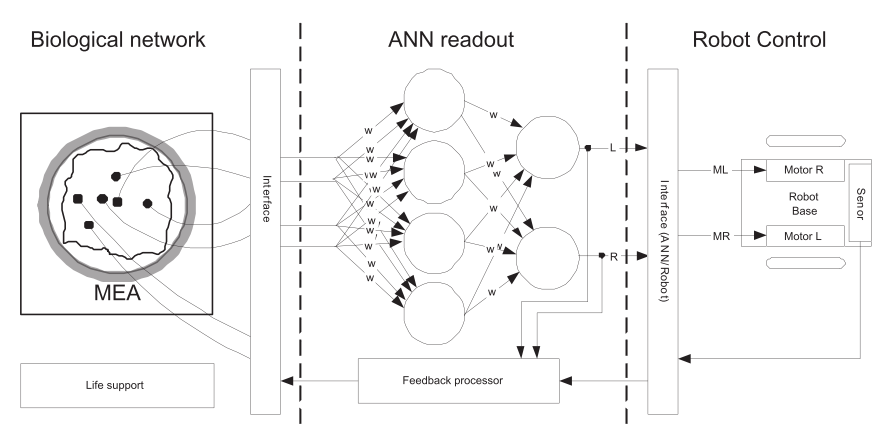
\includegraphics[width=\linewidth]{images/cyborg_overview.png}
    \caption{The gist of it..}
    \label{fig:cyborg_idea}
\end{figure}
\subsubsection{Growing NIV}
\subsubsection{A First Test}


\subsection{MEA2100}
To perform experiments a MEA2100 system has been purchased from multichannel systems.
The MEA2100 system is built to conduct experiments on in-vitro cell cultures, 
with the main focus being on neurons.
The principal components of the MEA2100 systems are:
\subsubsection{Micro electrode array}
\begin{figure}[h!]
    %\centering
    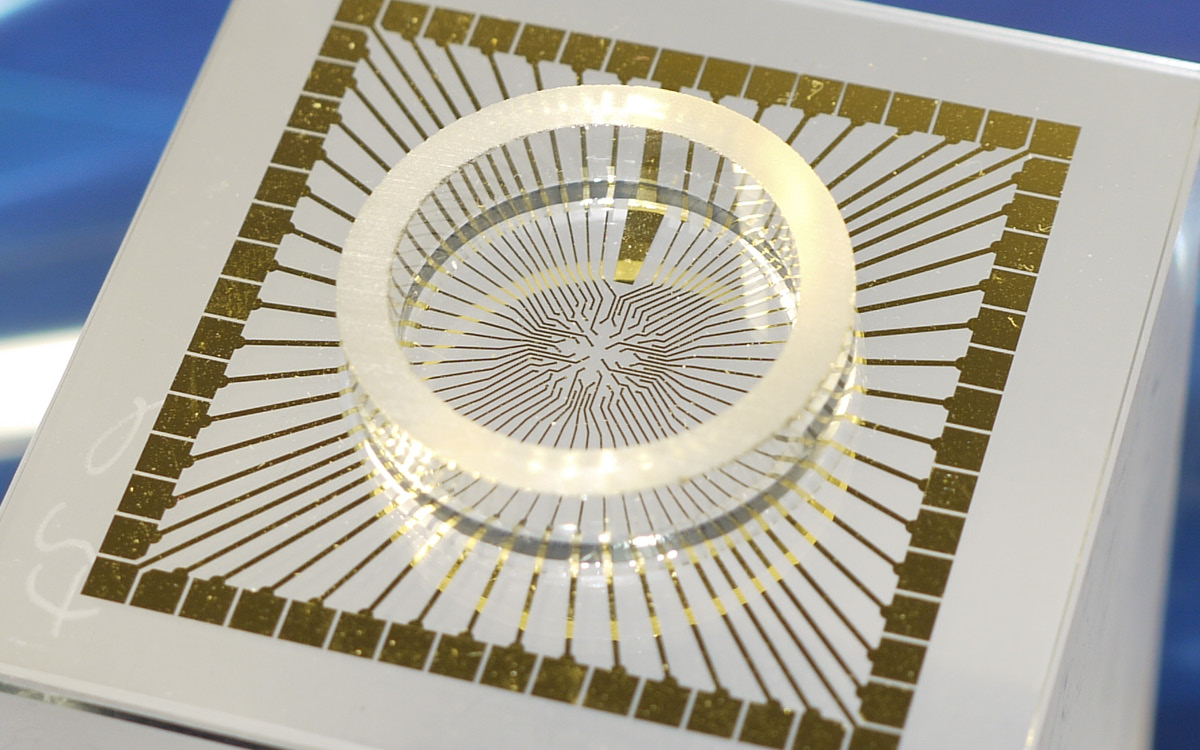
\includegraphics[width=\linewidth]{images/MEA.jpg}
    \caption{A generic MEA}
    \label{fig:generic_MEA}
\end{figure}
To experiment on the properties of cells or other electrically active subjects the
micro electrode array (MEA) is used. As the name implies the MEA is equipped with
an array of electrodes able to both measure the electrical properties of the 
experiment subjects, as well as applying outside stimuli, acting in a sense as
output and input for the subject. \ref{fig:generic_MEA} shows an empty MEA,
\ref{st_olav_MEA} shows an MEA from st.olavs with a live neuron culture.
\begin{figure}[h!]
    %\centering
    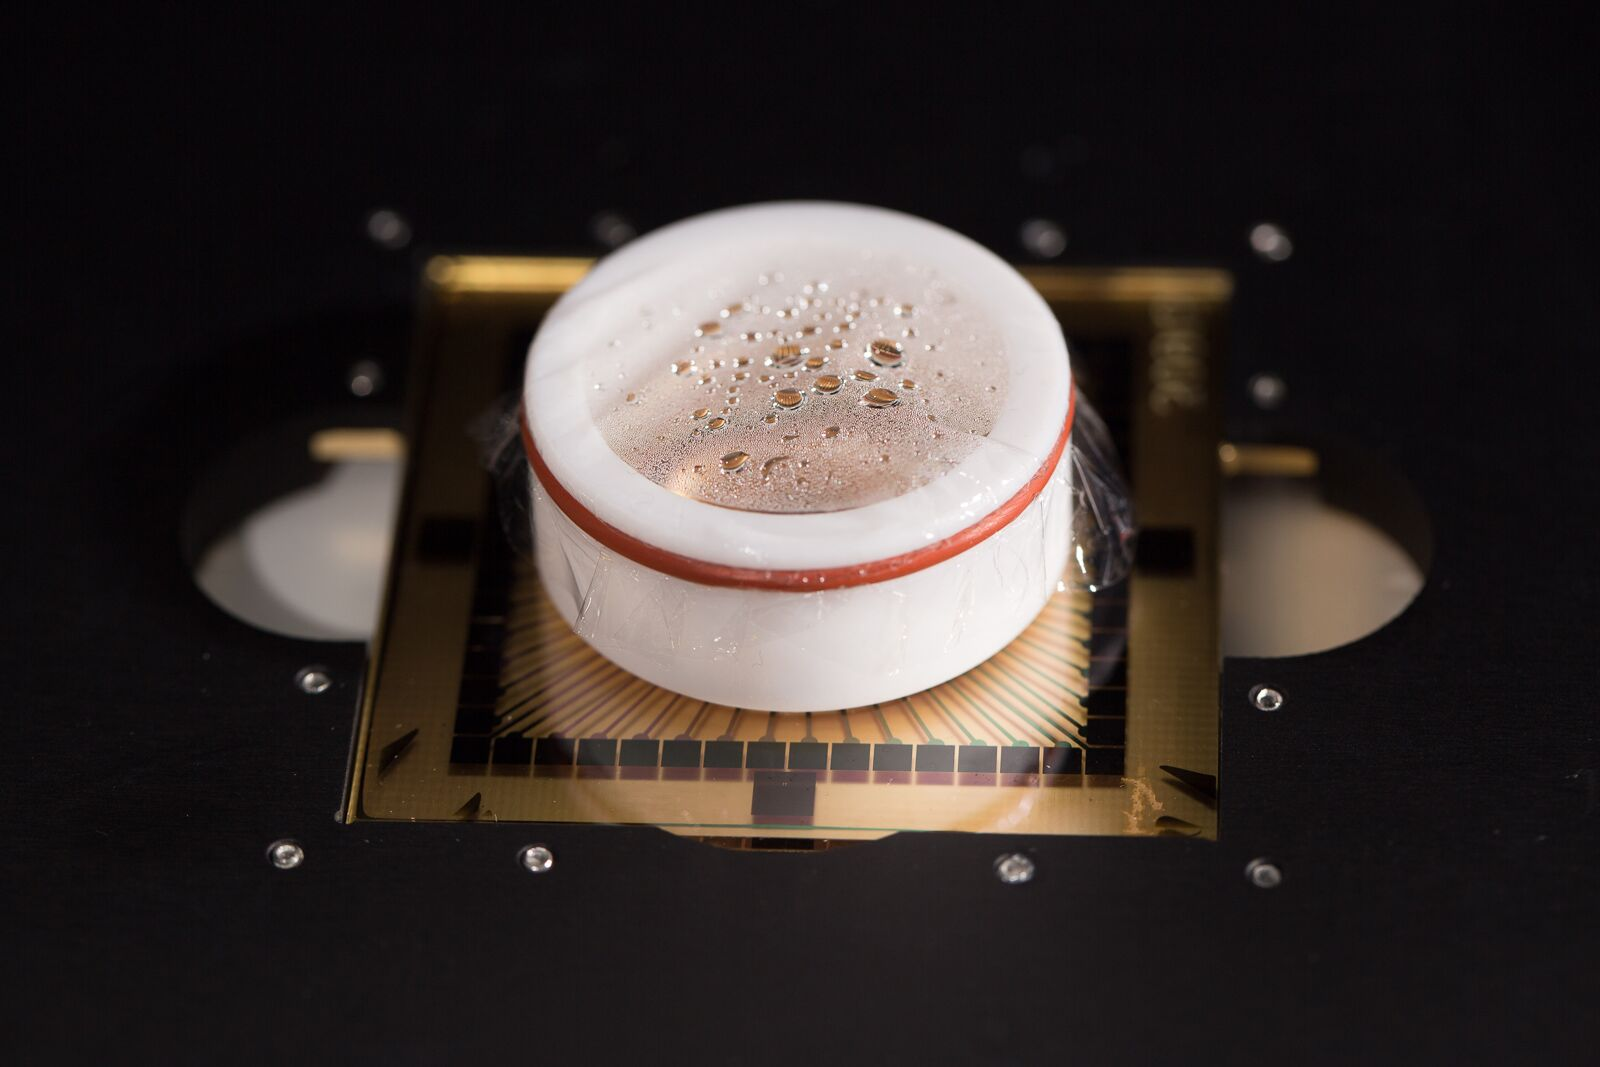
\includegraphics[width=\linewidth]{images/st-olavs-mea.jpg}
    \caption{A MEA with a live culture, photographed by Kai}
    \label{fig:st_olav_MEA}
\end{figure}
\subsubsection{Headstage}
The electrodes of the MEAs are measured and stimulated by the headstage which
contains the necessary high precision electronics needed for microvolt range readings.
\ref{fig:headstage} shows the same type of headstage used in this paper along
with an MEA.
\begin{figure}[h!]
    %\centering
    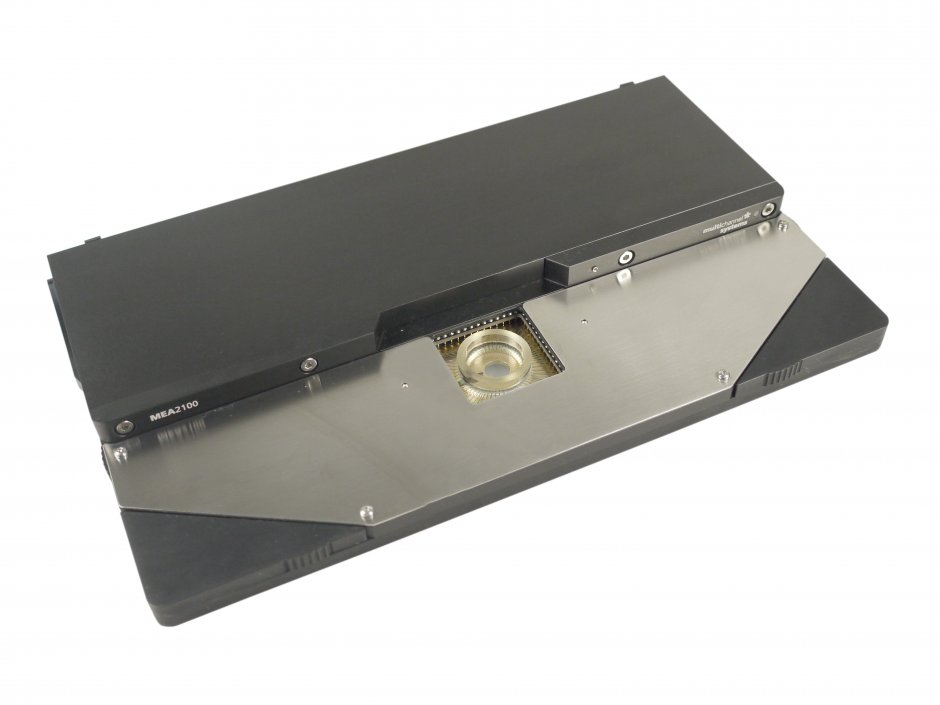
\includegraphics[width=\linewidth]{images/MEA2100-HS60.jpg}
    \caption{The headstage}
    \label{fig:headstage}
\end{figure}
\subsubsection{Interface board}
The interface board connects to up to two head-stages and is responsible for interfacing
with the data acquisition computer, as well as auxiliary equipment such as temperature
controls.
\begin{figure}[h!]
    %\centering
    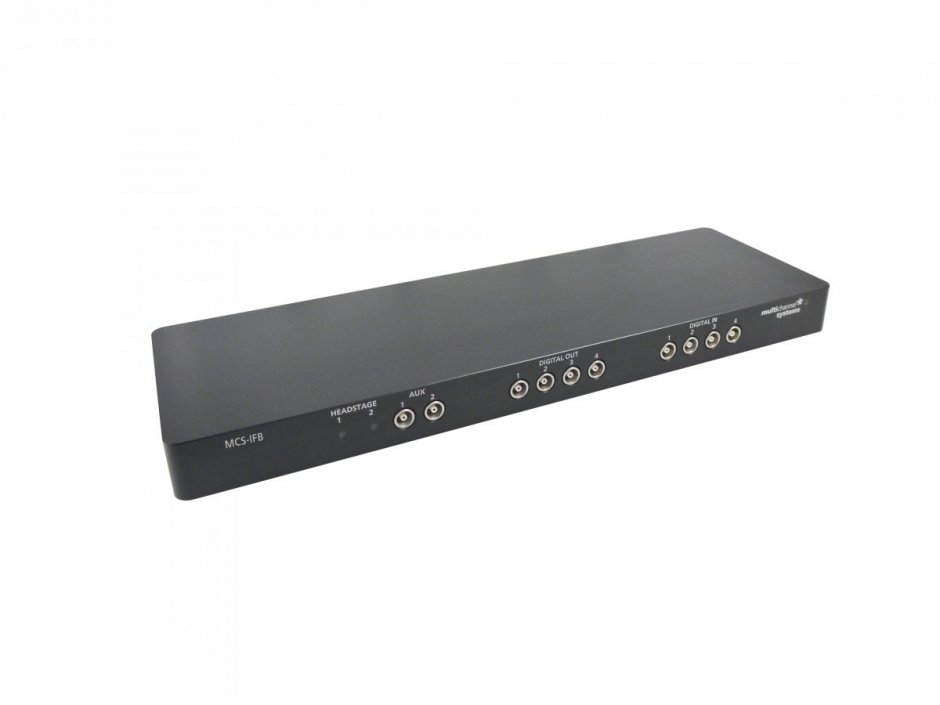
\includegraphics[width=\linewidth]{images/MCS-IFB.jpg}
    \caption{The MCS interface board}
    \label{fig:neuron_anatomy}
\end{figure}
The interface board has two modes of operation.
In the first mode the interface board processes and filters data from up to two
headstages as shown in \ref{fig:IFB_regular} which can then be acquired on a normal
computer connected via USB.
In the second mode of operation a Texas instruments TMS320C6454 digital signal
processor is activated which can then be interfaced with using the secondary USB
port as shown in \ref{fig:IFB_BSP}
\begin{figure}[h!]
    %\centering
    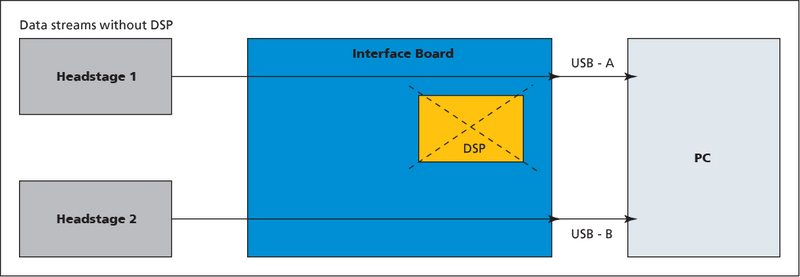
\includegraphics[width=\linewidth]{images/regular_operation.png}
    \caption{Casual mode}
    \label{fig:IFB_regular}
\end{figure}
%% %% %% %% %% %% %% %% %% %% %% %% %% %% %% %% %% %% %% %% %% %% %% %% %% %%
%% %% %% %% %% %% %% %% %% %% %% %% %% %% %% %% %% %% %% %% %% %% %% %% %% %%
%% %% %% %% %% %% %% %% %% %% %% %% %% %% %% %% %% %% %% %% %% %% %% %% %% %%
%% %% %% %% %% %% %% %% %% %% %% %% %% %% %% %% %% %% %% %% %% %% %% %% %% %%
\begin{figure}[h!]
    %\centering
    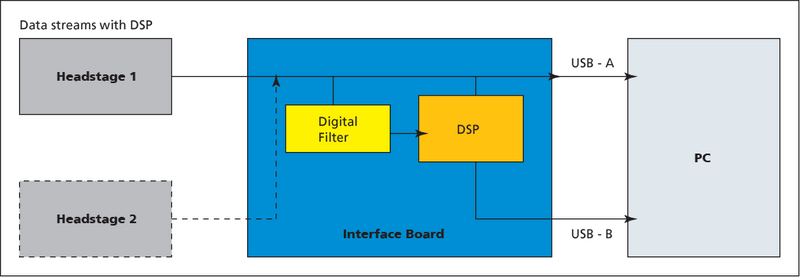
\includegraphics[width=\linewidth]{images/dsp_operation.png}
    \caption{DSP active}
    \label{fig:IFB_DSP}
\end{figure}
%% %% %% %% %% %% %% %% %% %% %% %% %% %% %% %% %% %% %% %% %% %% %% %% %% %%
%% %% %% %% %% %% %% %% %% %% %% %% %% %% %% %% %% %% %% %% %% %% %% %% %% %%
%% %% %% %% %% %% %% %% %% %% %% %% %% %% %% %% %% %% %% %% %% %% %% %% %% %%
%% %% %% %% %% %% %% %% %% %% %% %% %% %% %% %% %% %% %% %% %% %% %% %% %% %%
\begin{figure*}[p]
    \centering
    \includegraphics[width=\textwidth]{images/"Neuron anatomy".png}
    \caption{a neuron}
    \label{fig:neuron_anatomy}
\end{figure*}
%%% Local Variables:
%%% mode: latex
%%% TeX-master: "../main"
%%% End:
